\documentclass[11pt]{article}

\usepackage[utf8]{inputenc}
\usepackage[T1]{fontenc}
\usepackage{amsmath,amssymb,amsthm}
\usepackage{hyperref}
\usepackage{graphicx}
\usepackage{geometry}
\geometry{margin=2.5cm}
\usepackage{tikz}
\usepackage{pgfmath}
\usepackage{mathtools}

\newtheorem{theorem}{Theorem}

\theoremstyle{definition}
\newtheorem{definition}{Definition}[section]

\title{Trigonometry without $\pi$: A Constructive Approach}
\author{Daniel de Rauglaudre}
\date{\today}

\begin{document}

\maketitle

\begin{abstract}
We present a construction of trigonometry in which angles are not real
numbers, but pairs $(x,y)$ satisfying $x^2 + y^2 = 1$. Several
classical trigonometric formulas naturally emerge during this
construction, leading to the definition of angle division by natural
numbers via a convergent sequence. Notably, this approach does not
rely on the prior definition of the constant $\pi$, which is never
used. All results are rigorously proven using the Rocq proof assistant
(formerly known as Coq), but no prior knowledge of Rocq is required to
read this paper, as no Rocq code appears.
\end{abstract}

\section{Introduction}

The title \emph{trigonometry without $\pi$} might sound a bit
clickbait, and we admit it is. It's hard to imagine how one could do
trigonometry without $\pi$: a right angle is $\pi/2$, angles are often
defined up to $2k\pi$, formulas involve things like $\cos(x + \pi/2)$,
and even physicists write $\hbar/2\pi$, $2\pi\varepsilon_0$ and all
that sort of things. As soon as something rotates, $\pi$ shows up.

This work does not aim to replace $\pi$ with degrees or grads. It’s
just a different approach, one in which $\pi$ does not appear—not
because we tried to eliminate it, but because we simply didn’t need
it.

The main goal is to present a construction of trigonometry that allows
us to recover some classical formulas, and that leads—this is the real
point—to dividing an angle by a natural number. This turns out to be
less trivial than it sounds, given the framework we adopt.

\medskip

\noindent\textbf{Disclaimer.} Trigonometry has been around for
centuries, if not millennia. I do not claim to have discovered
anything groundbreaking.  What I present here may well have been
thought of before. I'm not a specialist, and a web search turns up
thousands of pages that all say more or less the same thing. It’s hard
to find sources that stray from the standard path.

So, this work is not necessarily original in content. What may be more
original is the fact that it has been formalized it as a proof, in
Rocq.

\medskip

There is, however, something vaguely similar to my approach: Norman
Wildberger’s \emph{rational trigonometry}
(2005)~\cite{wildberger2005divine}. But there are three key
differences.

First, Wildberger avoids the word \emph{angle} altogether; he reserves
it for classical trigonometry, and instead uses the term
\emph{spread}. In contrast, I do use the word \emph{angle}, but with a
different definition.

Second, Wildberger rejects the square root, which makes sense if one
wants to stick to rational numbers. He avoids expressions like
$\sqrt{2}/2$, the cosine of $45^\circ$ or $\pi/4$, and works with
\emph{quadrance}, the square of the distance: $x^2 + y^2$ rather than
$\sqrt{x^2 + y^2}$. We, on the other hand, not only accept square
root, we use it in this approach, as we are going to see further.

Third, one of Wildberger’s goals is computational efficiency: rational
arithmetic is faster than floating-point. Personally, I don’t care. I
prefer doing pure math. What matters to me is that the construction is
provable, proved, and holds up logically.

\medskip

For those familiar with the Rocq proof assistant, I decided not to use
MathComp and instead developed my own implementation, based on my own
approach of mathematics.

\section{Why trigonometry?}

Why trigonometry? It is not that I am especially interested in the
subject, but I needed, in one of my proofs, to show that every complex
number $x+iy$ has an $n$th-root, for every nonzero integer $n$.

\bigskip \noindent How is that done? The trick is well known: one
writes the complex number $x+iy$ in polar form:
\[
x+iy=\rho\,e^{i\theta},
\]
and then the answer is immediate:
\[
\sqrt[n]{x+iy}=\sqrt[n]{\rho}\;e^{i\theta/n}.
\]

Here, the left-hand part of the right member is the $n$th-root of a
nonnegative real number, and not of a complex number. In the context
of my work, the existence of such a root can be assumed as an
axiom. What remains is the right-hand part.

On the right, we have $\theta$, an angle. Hence, trigonometry. And
this angle must be divided by an integer. At first, I thought that one
had to introduce the exponential function, and, since according to
Euler
\[
e^{i\theta}=\cos\theta+i\sin\theta,
\]
also the sine and cosine functions, all defined by power series.

\bigskip \noindent However, I recalled one of my previous proofs: the
Banach--Tarski paradox~\cite{derauglaudre:hal-01673378}. In that
proof, there are rotations in every direction, and rotations involve
angles, sine, and cosine. I noticed, while coding that proof in Rocq,
that I often ended up with definitions and theorems where the pair
$(\cos\theta,\sin\theta)$ appeared either as parameters or as
hypotheses. But I realized that, in essence, I did not care that it
was an angle; I did not need sine and cosine. It was much simpler to
use pairs $(x,y)$ with $x^2+y^2=1$, thereby ignoring traditional
trigonometry and all its business.

Later, in that proof I indeed had to use $\cos$ and $\sin$, but for a
large part of it the pairs $(x,y)$ satisfying $x^2+y^2=1$ were
sufficient.

\bigskip \noindent So for this work, we decided to see if this approach
could be defined systematically.

\section{Basic Construction}

\subsection{Angles}

In classical trigonometry, angles are real numbers. The set \( A \) of
angles is therefore defined by
\[
A ::= \mathbb{R}
\]

\noindent Here, we set aside this definition and instead define:
\[
A ::= \{ \; (x, y) \; | \; x^2 + y^2 = 1 \; \}
\]

\noindent In other words, an angle is defined by a point on the unit
circle.  This point represents the angle between the positive \( x
\)-axis and the line segment from the origin \( O \) to the point.

\medskip

\noindent The angle \( (x, y) \) is illustrated below:

\medskip

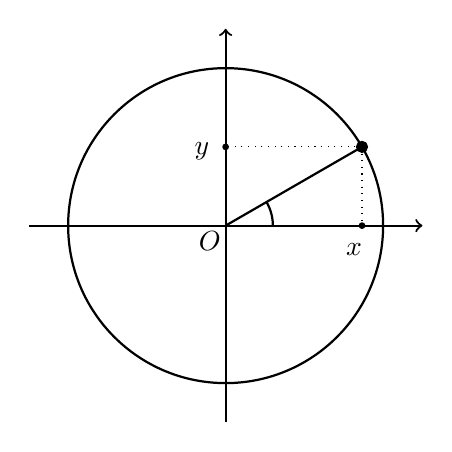
\begin{tikzpicture}
    \draw[thick] (0,0) circle(2);
    \draw[->, thick] (-2.5, 0) -- (2.5, 0);
    \draw[->, thick] (0, -2.5) -- (0, 2.5);
    \node at (-0.2,-0.2) {$O$};

    \pgfmathsetmacro{\px}{cos(30)}
    \pgfmathsetmacro{\py}{sin(30)}
    \coordinate (P) at (\px*2, \py*2);
    \draw[fill] (P) circle (2pt);
    \draw[thick] (0,0) -- (P);
    \draw[thick] (0.6,0) arc[start angle=0, end angle=30, radius=0.6];

    \draw[dotted] (P) -- (\px*2, 0);
    \draw[fill] (\px*2, 0) circle (1pt);
    \node at ({\px*2 - 0.1}, -0.3) {$x$};

    \draw[dotted] (P) -- (0, \py*2);
    \draw[fill] (0, \py*2) circle (1pt);
    \node at (-0.3, {\py*2 - 0.05}) {$y$};
\end{tikzpicture}

\medskip

\noindent In our setting, an angle \( \theta \) is not a real number,
but a triple of the form
\[
\theta = (x, y, p),
\]
where \( (x, y) \in \mathbb{R}^2 \), and \( p \) is a proof (or
witness) that \( x^2 + y^2 = 1 \); we define:
\[
cos(\theta) \coloneqq x, \qquad sin(\theta) \coloneqq y.
\]

\noindent While in classical mathematics, cosine and sine are defined
by power series, here they are just the first two components of the
triplet.  The theorem:
\[
cos^2(\theta) + sin^2(\theta) = 1
\]
is true by definition: its proof is \( p \), the third component of
the triplet.

\subsection{Notations}

In the following, we sometimes represent an angle just as the pair \(
(x, y) \), the third component being implicit. Also, even if the
constant $\pi$ is not required, we use it as a notation to represent
some angles, as follows:
\[
\begin{array}{rll}
\pi/2    &:= (0, 1) & \hspace{1em} \text{the right angle} \\
\pi      &:= (-1, 0) & \hspace{1em} \text{the straight angle}
\end{array}
\]

\noindent we also write
\[
\theta_1 + \theta_2 < 2\pi
\]
to express
\[
\text{``the sum of these angles is less than one turn''}
\]

\medskip

\noindent These notations are purely symbolic: they are shortcuts for
angles, not expressions involving the real constant \( \pi \).

\subsection{Drawback}

The difficulty arises from the arithmetic of angles. In classical
trigonometry, this issue does not appear, since angles are treated as
real numbers. Any operation that is defined on the reals—addition,
subtraction, multiplication, division, and so on—is directly
applicable to angles.

However, when we think of angles as points on the unit circle, we can
no longer rely on the standard algebraic operations. These points, in
themselves, do not carry any inherent arithmetic structure. In order
to define such operations, we must construct them from scratch. We
begin with addition in the next section.

\section{Addition of angles}

If we have two angles $(x, y)$ and $(x', y')$, we want to define an
addition, giving a third angle $(x'', y'')$, such that
$x''^2+y''^2=1$.
\[
(x, y) + (x', y') ::= (x'', y'')
\]

\medskip

\noindent The solution comes from normal trigonometry. If we have two
angles $a$ and $b$, we know that
\[
cos(a+b) = cos\;a\;.\;cos\;b - sin\;a\;.\;sin\;b
\]
\[
sin(a+b) = sin\;a\;.\;cos\;b + cos\;a\;.\;sin\;b
\]

\medskip

\noindent In our trigonometry, if we consider that the angle $(x, y)$
is ``$a$'', and the angle $(x', y')$ is ``$b$'', the angle $(x'',
y'')$ is ``$a + b$''. Applying the classical formulas above, we can
define the addition of angles as
\[
(x, y) \boldsymbol{+} (x', y') \coloneqq (x x' - y y', x y' + y
x').
\]
and we can prove that the sum of the squares of the RHS is indeed
$1$. This is a consequence of the fact that $x^2+y^2=1$ and
$x'^2+y'^2=1$. The two classical formulas above, about $cos(a+b)$ and
$sin(a+b)$, are now true by definition of $+$.

\section{Additive group}
\label{angle_add_group}

Addition of angles is trivially commutative, and associativity can
also be proven. The neutral element is $(1, 0)$, the null angle. It
says that $cos\;0=1$ and $sin\;0=0$. The inverse element of $(x, y)$
is $(x, -y)$, expressing that $cos\;(- \theta) = cos\;\theta$ and
$sin\;(- \theta) = - sin\;\theta$. All these values and formulas are
what we find in normal trigonometry.

\medskip

\noindent Like for all additive groups, it is possible to define
external multiplication by a natural $n$, by adding the element $n$
times:
\[
  n \; \theta ::=
  \underbrace{\theta + \theta + ... + \theta}_{n \; \text{times}}
\]

\subsection*{And multiplication?}

What about {\em multiplication} of two angles? In our framework, it
seems not possible. Because {\em addition} of angles is actually {\em
  multiplication} of complex numbers. Perhaps, then, multiplication of
angles could be something that {\em exponentiation} of complex
numbers? But this intuition seems not to work.

Moreover, as far as geometry is concerned, multiplication of angles
seems to have no meaning. In this work, we didn't define it.

This has a consequence: it is not possible to define exponentiation of
imaginary angles either, which we found in the famous expression
$e^{i\theta}$ of classical trigonometry, supposed to be equal to
$cos\;\theta+i\;sin\;\theta$ (Euler's formula), because
exponentiation is defined by a power series holding powers of its
parameter:
\[
e^x = \sum_{n=0}^\infty{\; \frac{x^n}{n!}}
\]

\noindent i.e. its parameter $x$ {\em multiplied} several times by
itself. Since multiplication of angles doesn't exist, Euler's formula
doesn't work, but we see further, that de Moivre's formula works in
our trigonometry and we use it. Remainder: de Moivre's formula is:
\[
(cos \; \theta + i \; sin \; \theta)^n = cos (n \theta) + i \; sin (n
\theta)
\]

\medskip

\noindent But what we need, for the moment, is division by a
natural. We defined above multiplication by a natural. Division is
more complicated but we see in next sections that it is possible to
define it.

\section{Trying to define the division of an angle by a natural}

Starting with de Moivre's formula (stated above), which is easily
provable by induction to $n$, and supposing we already have a division
of an angle by a natural, we can apply it with $\theta / n$ and get:
\[
(cos \left(\frac{\theta}{n}\right) + i \; sin
\left(\frac{\theta}{n}\right))^n = cos \; \theta + i \; sin \;
\theta
\]

\noindent Warning: it doesn't mean that $\theta / n$ exists. But, if
it exists, it must fit this equation. Let's rewrite the equation with
simple variables. Since $cos\;(\theta/n)$ and $sin\;(\theta/n)$ are
our unknowns, let's name them $x$ and $y$, and since $cos\;\theta$ and
$sin\;\theta$ are our data, let's name them $u$ and $v$, and we have
to resolve:
\[
(x + i \; y)^n = u + i \; v
\]

\noindent If we develop the power to $n$, we get a complex number
whose real and imaginary part are polynomials of degree $n$
respectively in $x$ and in $y$. In general, we have no formulas to
resolve these equations for all $n$.

\medskip

\noindent But we can resolve it for $n=2$, i.e. for:
\[
(x + i \; y)^2 = u + i \; v
\]

\noindent and it will give us the way to compute $\theta/2$.

\section{Division of an angle by 2}
\label{angle_div_2}

Resolving this equation, and knowing that the angle $(x, y)$ is
actually the angle $(u, v)/2$, we get a realistic definition of the
division of an angle by 2:
\[
\displaystyle \frac{(u, \; v)}{2} ::=
\left( \sigma (v) \sqrt{\frac{1 + u}{2}}, \;
\sqrt{\frac{1 - u}{2}} \; \right)
\]

\noindent where $\sigma(v)$ is the {\em sign} of $v$. We can compute
twice the right hand part, i.e. the right hand part {\em plus} the
right hand part, using our definition of addition, and we get $(u, v)$
back. This definition of the division of the angle by 2 is therefore
reasonable.

\medskip

\noindent But we need a division of an angle by any $n$, not only by
2. How to do that? To answer this question, let's see, in next
section, a method to divide the natural 1 by another natural, a normal
division with decimals. In that section, we temporarily forget the
fact that we work with angles. We return to angles the section after
that one.

\section{Division by a natural}

Let's divide 1 by $n$, i.e. take the inverse of $n$. If we do the
division in binary, we get something like:
\[
1 / n = 0.a_1a_2a_3...
\]

\noindent where the $a_k$ are bits, 0 or 1, since we decided to divide
in radix 2. Examples from 2 to 5:
\[
1 / 2 = 0.10000000...
\]
\[
1 / 3 = 0.01010101...
\]
\[
1 / 4 = 0.00100000...
\]
\[
1 / 5 = 0.00110011...
\]

\noindent and so on. But this representation with this decimal dot
and the list of digits is actually a syntax for the mathematical
expression:
\[
\displaystyle \sum_{k=1}^\infty{\; \frac{a_k}{2^k}}
\]

\noindent If we were in base 10, as we usually and generally do, we
would have to put $10^k$ in the denominator, instead of $2^k$.

\medskip

\noindent So, we have:
\[
\displaystyle 1 / n = 0.a_1a_2a_3... =
\sum_{k=1}^\infty{\; \frac{a_k}{2^k}}
\]

\noindent Now, we claim that:
\[
a_k = \left\lfloor \frac{2^k}{n} \right\rfloor {\scriptstyle mod \; 2}
\]

\noindent Indeed, starting with $1/n =
0\;.\;a_1\;a_2\;a_3\;...\;a_k\;a_{k+1}\;...$, \\
we have, $2^k/n = a_1\;a_2\;a_3\;...\;a_k\;.\;a_{k+1}\;...$
\\
Therefore its integer part, $\lfloor 2^k/n \rfloor$, is
$a_1\;a_2\;a_3\;...\;a_k$ \\
and its last digit, $a_k$, is this value $mod\;2$.

\bigskip

\noindent In short:
\[
\displaystyle 1 / n = \sum_{k=1}^\infty{\;
  \frac{a_k}{2^k}} \hspace{2.5em} \text{where} \hspace{0.5em} a_k =
\left\lfloor \frac{2^k}{n} \right\rfloor {\scriptstyle mod \; 2}
\]

\medskip

\noindent End of this parenthesis without angles. Let's return to
them.

\section{Trying to define the division of an angle by a natural}

In the previous formula, if we change the natural 1 into an angle
$\theta$, that gives a possible definition of an angle divided by a
natural:
\[
\frac{\theta}{n} ::= \sum_{k=1}^\infty \frac{a_k \; \theta}{2^k}
\hspace{2.5em}
a_k = \left\lfloor \frac{2^k}{n} \right\rfloor \bmod 2
\]

\noindent We claim that this formula is indeed composed of operations
on angles that we know how to perform.

\begin{itemize}
\item Inside the sum, the expression $a_k \; \theta$ is an angle
  multiplied by a natural; we said above
  (section~\ref{angle_add_group}) that we know how to do that; by the
  way, $a_k$ being a bit, this is simply the null angle if $a_k=0$ or
  the angle $\theta$ itself if $a_k=1$.
\item We built a way to divide an angle by 2
  (section~\ref{angle_div_2}), so it is possible to divide it by
  $2^k$, by repeating the operation $k$ times.
\item Therefore, the current term of the summation is an angle; since
  we have a sum of angles, we have a summation, provided we can define
  limits of sequences.
\end{itemize}

\noindent The next step is to prove that this power series converges.
For that, we define the sequence of this power series up to some
natural $m$:
\[
\theta_m ::= \sum_{k=1}^m \frac{a_k \; \theta}{2^k}
\]

\noindent and prove that this sequence converges when $m$ tends to
infinity. But before doing that, using the formula for $a_k$, it is
possible to prove that, in fact, $\theta_m$, the partial sum up to
$m$, is simply equal to:
\[
\theta_m ::= \left\lfloor \frac{2^m}{n} \right\rfloor \frac{\theta}{2^m}
\]

\noindent By the way, if we look at this much simpler formula, we see
that $2^m$ appears in both the numerator and denominator. Of course,
we cannot simplify it, but if we do so intuitively, just to see, we
note that what remains is $\theta / n$.

\medskip

\noindent Since we are in a case where there is no closed formula for
the limit, we:

\begin{itemize}
\item proved that $(\theta_m)$ is a Cauchy sequence;
\item proved that the set of angles is complete.
\end{itemize}

\noindent Since we have these properties, we are allowed to consider
\[
\theta' = \lim_{m \rightarrow \infty} \theta_m
\]

\noindent and we proved that this $\theta'$ satisfies $n\theta' =
\theta$, which is a reasonable property for something supposed to be
$\theta / n$.

\medskip

\noindent Now, replacing $\theta_m$ by its value, we decided to define
$\theta / n$ as:

\[
\boxed{
  \frac{\theta}{n} ::= \lim_{m \rightarrow \infty}
  \left\lfloor \frac{2^m}{n} \right\rfloor \frac{\theta}{2^m}
}
\]

\medskip

\noindent and a proof that $n(\theta/n)=\theta$ is available in the
code.

\section{Difficulties}

We don't give the detail of all these proofs, it would be rather long,
it could require a paper by itself, and they are accessible in the
sources, anyway. But we met several difficulties. We cite the most two
important ones.

\medskip

\noindent A notable challenge comes from the fact that in our
trigonometry, when adding two angles, the properties may change
if this sum exceeds a turn.

\subsection{First difficulty}

We had to prove that:
\[
\frac{\theta_1 + \theta_2}{2} = \frac{\theta_1}{2} + \frac{\theta_2}{2}
\]

\medskip

\noindent This seems obvious, and it is when angles are real numbers,
but in our trigonometry, it is not. We must consider the 4 quadrants
of $\theta_1$ and the 4 quadrants of $\theta_2$, i.e. 16 cases. All
cases are different and we didn't find common rules or lemmas, that
could have made this proof easier.

\medskip

\noindent Moreover, this proof is cursed by the malediction above,
i.e. when the sum $\theta_1+\theta_2$ exceeds one turn, we must add
the straight angle in the right hand side. The correct formula is
actually:
\[
\frac{\theta_1 + \theta_2}{2}\hspace{0.5em} = \hspace{0.5em}
\left\{
\begin{array}{ll}
  \displaystyle \frac{\theta_1}{2} + \frac{\theta_2}{2}
    & \hspace{1em} \text{if } \theta_1 + \theta_2 < 2 \pi \\
  [1em]
  \displaystyle \frac{\theta_1}{2} + \frac{\theta_2}{2} + \pi
    & \hspace{1em} \text{otherwise}
\end{array}
\right.
\]

\noindent A way to see the problem is to look at the case when
$\theta_1 = \theta_2 = \pi$. We see that the LHS is $0$ but the RHS is
$\pi$. Adding $\pi$ in that case returns to $0$. The 16 cases of the
proof therefore became 32 cases.

\subsection{Second difficulty}

We had to prove that:
\[
\theta_1 + \theta_3 \le \theta_2 + \theta_3 \; \Rightarrow \; \theta_1
\le \theta_2
\]

\medskip

\noindent Three angles, this time, i.e. 64 cases, times the cases of
sum of angles exceeding a turn.

\section{Further directions}

After the construction of the division of angles by a natural, we tried
out to see if this approach of trigonometry could go further.

\medskip

\noindent However, these developments lie outside the scope of this
article. We just mention them here.

\subsection{Derivation}

We have defined a notion of limit and differentiability, allowing
proofs of the classical results such as $cos'=-sin$, $sin'=cos$, and
$tan'=1/cos^2$. For this last case, we had to previously prove the
formulas of derivation of product and inverse.

\medskip

\noindent Note that, generally, derivation is for functions from
$\mathbb{R}$ to $\mathbb{R}$. Here, our functions cos, sin and tan are
from $\mathbb{U}$ (unit circle) to $\mathbb{R}$. This implies a good
definition of limits, continuity and derivability when the domain of
the function is $\mathbb{U}$.

\medskip

\noindent In fact, we made a general definition of limit when tending
to a neighbourhood for any functions whose domain is $A$ and codomain
is $B$ when both sets have a distance, and the set $A$ has a relation
order. So it can be used for any kind of function. This can be
described in another paper.

\subsection{Hyperbolic trigonometry}

Also, we defined hyperbolic trigonometry, where hyperbolic angles are
on the hyperbole, i.e. points $(x, y)$ such that $x^2-y^2=1$, allowing
to define $cosh$ and $sinh$. The definition must include the condition
$x>0$, because hyperbolic functions only work for the right branch of
the hyperbole.

\subsection{Other formulas}

Of course, there is the matter of proving additional trigonometric
formulas. Although we have not done so because they were not needed,
they should be established. In one of our works, we also proved the
formula for $\cos p + \cos q$, which is not exactly the standard
version, as it depends on whether $p+q$ and $p-q$ exceed a full turn
or not.

\subsection{Nth roots of unity}

One can observe that dividing an angle by a natural number allows us
to define the $n$th root of unity. However, note that one must not
write $2\pi/n$, because in our construction $2\pi=0$, yielding only
the trivial root. The trick is to write $2(\pi/n)$, by parenthesizing
$\pi/n$ (which is important). Indeed, $\pi/n$ is nonzero.

\subsection{Lie groups}

One may also note that the unit circle is a Lie group, which seems to
be reflected in this construction. However, since my knowledge in this
area is limited, I cannot fully develop the consequences of
this.

\subsection{Exponential of an imaginary angle}

We have seen that it is impossible to define $e^{i\theta}$ in our
framework, since we do not have an exponential function due to the
fact that we cannot define the multiplication of angles. Moreover,
$i\theta$ is not an angle; it is an ``imaginary angle''. Yet, an
imaginary angle resembles a hyperbolic angle. In classical hyperbolic
trigonometry, we have
\[
e^a=\cosh a+\sinh a,
\]
which provides a definition of the exponential, and one can show that
$e^{a+b}=e^a\cdot e^b$, the well-known property of
exponentials. However, in this case, ``$a$'' denotes a hyperbolic
angle, that is, a pair $(x,y)$ such that $x^2-y^2=1$, which is not an
exponential on the reals as one might desire. One might define the
logarithm, but it would again yield a hyperbolic angle rather than a
real number.

\subsection{From normal trigonometry to trigonometry without $\pi$ and vice versa}

It is important to note that switching between normal trigonometry and
trigonometry without $\pi$ is straightforward.

\begin{itemize}
  \item If we are given an angle $\theta \in \mathbb{R}$ in the usual
    sense, we can represent it as the pair $(\cos \theta, \sin
    \theta)$ in our construction.
  \item Conversely, if we have a pair $(x, y)$ such that $x^2 + y^2 =
    1$, we can recover the "normal" angle by computing the arccosine:
    $\theta = \sigma(y) \; \text{acos}(x)$, where $\sigma(y)$ is the
    {\em sign} of $y$. This gives us an angle between $-\pi$ and
    $\pi$, as expected in traditional trigonometry.
\end{itemize}

\section{Conclusion}

This paper has presented a constructive approach to trigonometry,
where the notion of an angle is derived from the unit circle and its
geometric properties, without the need for a predefined constant like
$\pi$. Through the formalization in Rocq, we have shown that angle
division is possible within this framework, offering a new way of
understanding trigonometric relationships. While this approach is not
intended to replace traditional trigonometry, it provides an
alternative perspective that is grounded in formal reasoning and
geometric intuition.

The formalization of these concepts in Rocq has implications beyond
the immediate scope of trigonometry. It highlights the potential for
formal methods to reshape classical areas of mathematics, providing a
solid foundation for further exploration in both mathematical theory
and practical applications.

In this framework, $\pi$ is no longer a prerequisite — it is a derived
notation. Whether that makes trigonometry more elegant or more
unsettling is left to the reader’s taste.

\section{Acknowledgements}

I would like to express my sincere gratitude to Geoffroy Couteau
(CNRS), a leading expert in cryptography, for his invaluable
assistance in overcoming several proof challenges during the course of
this work. In particular, the formula for the convergent sequence
towards \(\theta/n\) was derived during one of our discussions, and I
am deeply grateful for his input. While his expertise is not directly
related to the mathematical content of this paper, his insights were
critical in advancing this project.

I am also thankful to my colleagues, who patiently listened to my
spontaneous visits in their offices, where I would often share my
formalization journey, discuss tricky proof obstacles, or simply
express my excitement over a newly proven lemma. Their curiosity,
support, and occasional mathematical insights created the kind of
collaborative environment where ideas can truly flourish.

\section{Source code}

\url{https://github.com/roglo/rocq_trigo_without_pi}

\bibliographystyle{alpha}
\bibliography{biblio}

\end{document}
